
\begin{figure}[H]%
    \centering
    \subfloat[Nube de puntos]{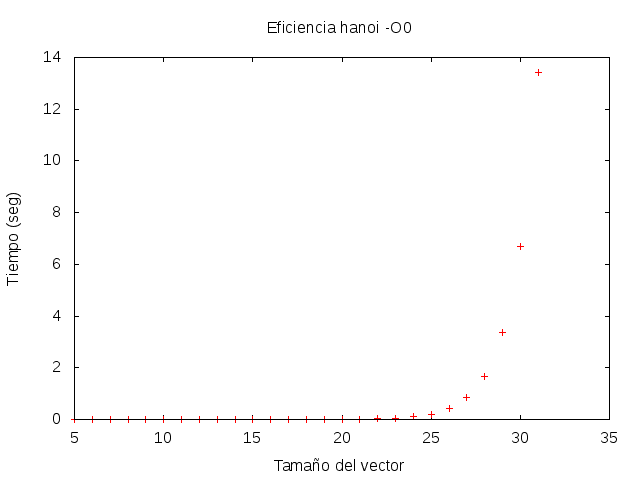
\includegraphics[width=0.5\textwidth]{../plots/hanoi_O0_points.png}}%
    \subfloat[Función continua]{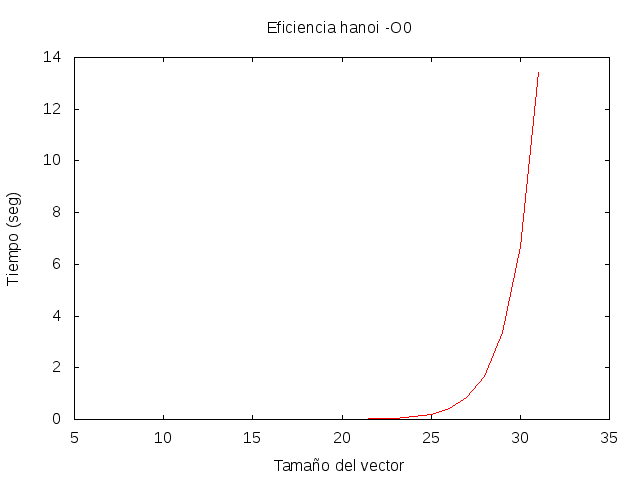
\includegraphics[width=0.5\textwidth]{../plots/hanoi_O0_lines.png}}%
    \caption{Resultados experimentales representados mediante una nube de puntos y la linea que los une}%
    \centering
    \subfloat{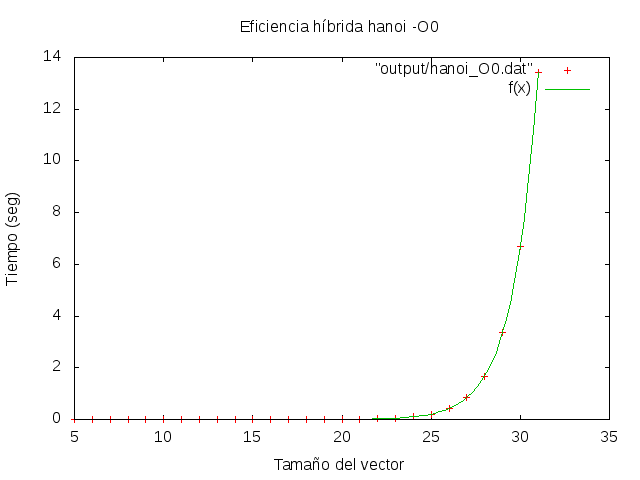
\includegraphics[width=0.6\textwidth]{../plots/hanoi_O0_fit.png}}%
    \caption{Ajuste para: calculo de los movimientos en las torres de hanoi}%
\end{figure}

\begin{verbatim}

\end{verbatim}
